% !TeX program = xelatex
% Build from the project root with build.ps1 -Document exercises/4/main.tex.
\documentclass[12pt,a4paper]{article}
\RequirePackage{array}[=2024-06-01]
% !TeX root = ../2/main.tex
\usepackage[a4paper,margin=25mm,headheight=16pt]{geometry}
\usepackage{amsmath,amssymb}
\usepackage{graphicx}
\usepackage{booktabs}
\usepackage{tabularx}
\usepackage{siunitx}
\usepackage{tikz}
\usepackage{circuitikz}
\usepackage[unicode,hidelinks]{hyperref}
\usepackage{xepersian}
% Only the regular B Nazanin file is installed; synthesize bold explicitly.
\settextfont[Path=C:/Windows/Fonts/,AutoFakeBold=2,AutoFakeSlant=0.2]{B-NAZANIN.TTF}
% B Nazanin lacks U+066A (Arabic percent), required by xepersian's digit setup.
% Arial covers the complete required digit/punctuation set; Persian prose remains B Nazanin.
\setdigitfont[Path=C:/Windows/Fonts/,BoldFont=arialbd.ttf,ItalicFont=ariali.ttf,BoldItalicFont=arialbi.ttf]{arial.ttf}
\setmathdigitfont[Path=C:/Windows/Fonts/,BoldFont=arialbd.ttf,ItalicFont=ariali.ttf,BoldItalicFont=arialbi.ttf]{arial.ttf}
\setlatintextfont{TeX Gyre Termes}
% B Nazanin does not contain the default itemize bullet and dash glyphs.
\renewcommand{\labelitemi}{\(\bullet\)}
\renewcommand{\labelitemii}{\(\circ\)}
\renewcommand{\labelitemiii}{\(\diamond\)}
\setlength{\parindent}{0pt}
\setlength{\parskip}{0.5em}
\linespread{1.25}
\newcommand{\exercise}[1]{\section*{تمرین #1}}
% !TeX root = ../2/main.tex
% Shared title page for every assignment.
% Change only \AssignmentNumber and \AssignmentDate in each main document.

\newcommand{\AssignmentNumber}[1]{\gdef\assignmentnumber{#1}}
\newcommand{\AssignmentDate}[1]{\gdef\assignmentdate{#1}}

\newcommand{\assignmentnumber}{---}
\newcommand{\assignmentdate}{---}

% Stable course metadata
\newcommand{\universityname}{دانشگاه صنعتی امیرکبیر}
\newcommand{\universityalias}{پلی‌تکنیک تهران}
\newcommand{\facultyname}{دانشکده مهندسی کامپیوتر}
\newcommand{\coursename}{طراحی مدارهای مجتمع پرتراکم پیشرفته}
\newcommand{\studentname}{محمد خلیلی اصل}
\newcommand{\instructorname}{دکتر مهدی صدیقی}

\newcommand{\MakeAssignmentCover}{%
  \begin{titlepage}
    \thispagestyle{empty}
    \centering
    \linespread{1}\selectfont

    \vspace*{0mm}
    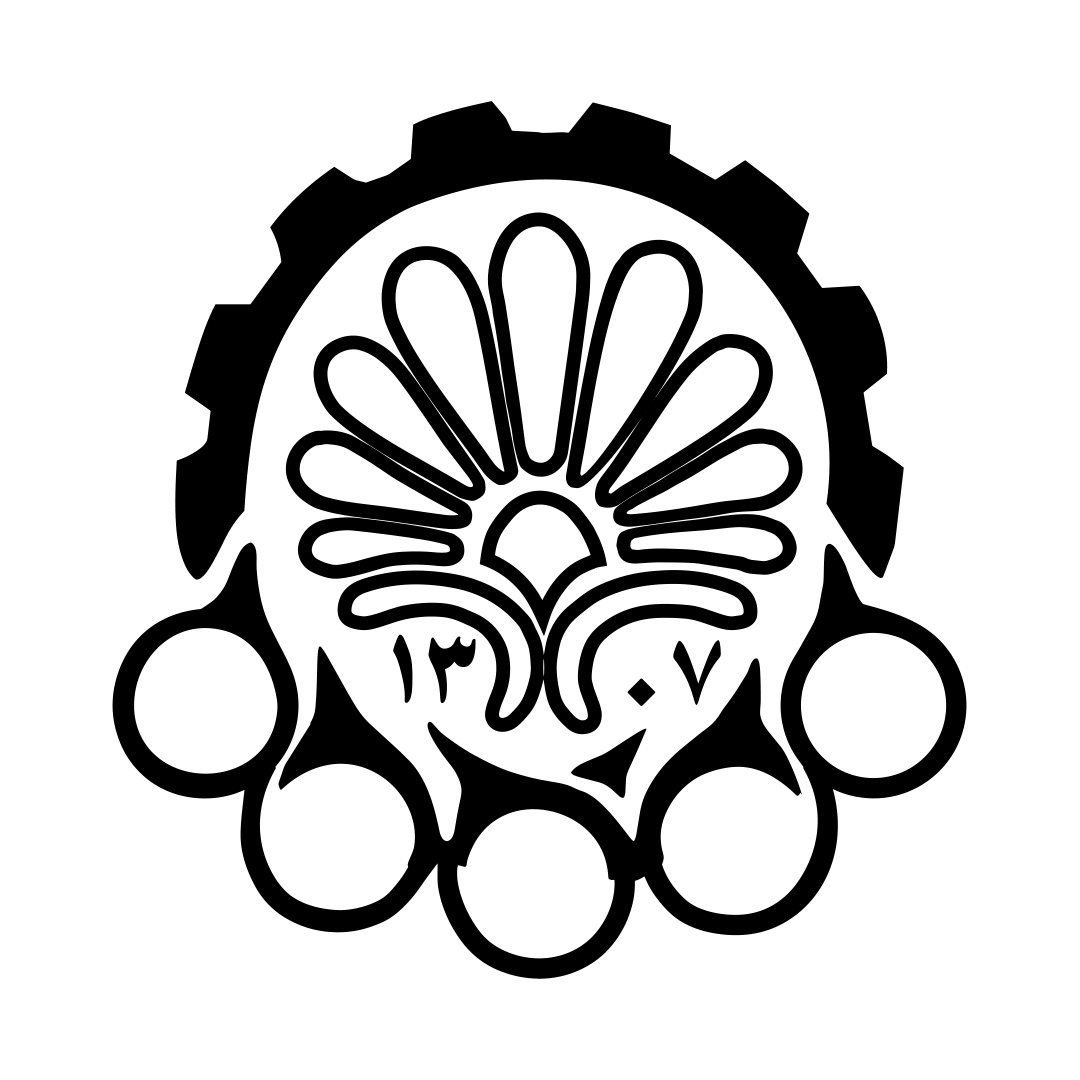
\includegraphics[width=44mm]{assets/aut-logo-black.png}\par
    \vspace{3mm}

    {\Large\bfseries \universityname\par}
    \vspace{1mm}
    {\large (\universityalias)\par}
    \vspace{1mm}
    {\large \facultyname\par}

    \vspace{8mm}
    {\Large\bfseries درس \coursename\par}

    \vspace{12mm}
    {\large عنوان\par}
    \vspace{2mm}
    {\LARGE\bfseries تمرین شماره \assignmentnumber\par}

    \vspace{10mm}
    {\large تهیه‌کننده\par}
    \vspace{2mm}
    {\Large\bfseries \studentname\par}

    \vspace{10mm}
    {\large استاد درس\par}
    \vspace{2mm}
    {\Large\bfseries \instructorname\par}

    \vspace{10mm}
    {\Large \assignmentdate\par}
    \vfill
  \end{titlepage}
  \setcounter{page}{1}%
}


\XeTeXgenerateactualtext=1
\newcommand{\secnum}[1]{\texorpdfstring{\mbox{\beginL#1\endL}}{#1}}
% Exercise titles already contain the original textbook numbers.
\setcounter{secnumdepth}{0}
\setlength{\emergencystretch}{3em}
\hypersetup{pdftitle={تمرینات فصل ۴},pdfauthor={محمد خلیلی اصل}}
\AssignmentNumber{تمرینات فصل ۴}
\AssignmentDate{}
\patchcmd{\MakeAssignmentCover}{تمرین شماره \assignmentnumber}{\assignmentnumber}{}{\errmessage{Cover title replacement failed}}

\begin{document}
\MakeAssignmentCover
\section{حل تمرین‌های \lr{Logical Effort}}
\label{sec:delay-exercises}

شماره‌های تمرین در این بخش از فصل \lr{Delay} کتاب گرفته شده‌اند.
مجموعه تمرین‌ها در اسلاید ۲۸ مشخص شده است. در حل‌ها، \(C\)
ظرفیت ورودی ترانزیستور واحد و \(R\) مقاومت مؤثر \lr{nMOS}
واحد است. مقاومت \lr{pMOS} واحد را \(2R\) می‌گیریم.
تأخیرها برحسب واحد مرجع \(\tau\) نرمال شده‌اند. در محاسبه‌های
عددیِ تأخیر \lr{Parasitic} از فرض \(p_{\mathrm{inv}}=1\)
استفاده می‌کنیم، مگر آنکه خود تمرین \(p_{\mathrm{inv}}\) را
به‌صورت پارامتر داده باشد
\cite[تمرین‌های \secnum{۴.۵} تا \secnum{۴.۱۰}، صفحه ۱۷۷]{weste}
\cite[اسلاید ۲۸]{logicaleffortslides}.

% !TeX root = ../main.tex
\subsection{تمرین \secnum{۴.۵}، مقایسه شیب و عرض از مبدأ}
\label{sec:delay-exercise-nor-plot}

\textbf{خواسته.}
نمودار تأخیر نرمال‌شده \lr{NOR} دوورودی را برحسب
\lr{Electrical Effort} رسم کنید و شیب و عرض از مبدأ را
با \lr{NAND} دوورودی مقایسه کنید
\cite[تمرین \secnum{۴.۵} و شکل \secnum{۴.۲۱}،
صفحات ۱۵۵ و ۱۷۷]{weste}.

\textbf{حل.}
محور افقی \(h=C_L/C_{\mathrm{in}}\) است که در آن \(C_L\)
ظرفیت بار خارجی و \(C_{\mathrm{in}}\) ظرفیت یک پایه ورودی
گیت است.
برای مقاومت راه‌اندازی برابر، ظرفیت ورودی هر پایه در
\lr{NOR2} برابر \(5C\) و در \lr{NAND2} برابر \(4C\)
است. ظرفیت ورودی \lr{Inverter} مرجع برابر \(3C\) است.
با تقریب ظرفیت‌های \lr{Diffusion} متصل به خروجی، هر دو
گیت \(p\approx2p_{\mathrm{inv}}\) دارند. بنابراین مدل خطی
دو رابطه زیر را می‌دهد.
\[
  d_{\mathrm{NOR2}}\approx\frac53 h+2p_{\mathrm{inv}},
  \qquad
  d_{\mathrm{NAND2}}\approx\frac43 h+2p_{\mathrm{inv}}.
\]
\begin{figure}[htbp]
  \centering
  \begin{latin}
  \begin{tikzpicture}[x=2.15cm,y=0.47cm]
    \draw[->] (0,0) -- (4.65,0) node[right] {\(h\)};
    \draw[->] (0,0) -- (0,9.05) node[above] {\(d\)};
    \node[below left] at (0,0) {\rl{۰}};
    \foreach \x/\ticklabel in {1/۱,2/۲,3/۳,4/۴} {
      \draw (\x,0.09) -- (\x,-0.09) node[below] {\rl{\ticklabel}};
    }
    \foreach \y/\ticklabel in {1/۱,2/۲,4/۴,6/۶,8/۸} {
      \draw (0.04,\y) -- (-0.04,\y) node[left] {\rl{\ticklabel}};
    }
    \draw[gray,densely dotted] (3,0) -- (3,7);
    \draw[thick] (0,1) -- (3.65,4.65) node[right] {\small Inverter};
    \draw[thick,blue!70!black,dashed] (0,2) -- (3.65,{2+3.65*4/3})
      node[right] {\small NAND2};
    \draw[thick,red!65!black,dashdotted] (0,2) -- (3.65,{2+3.65*5/3})
      node[right] {\small NOR2};
    \fill (3,4) circle (1.6pt);
    \fill[blue!70!black] (3,6) circle (1.6pt);
    \fill[red!65!black] (3,7) circle (1.6pt);
  \end{tikzpicture}
  \end{latin}
  \caption{تأخیر نرمال‌شده \(d\) برحسب \lr{Electrical Effort}
  بی‌بعد \(h\)، با فرض \(p_{\mathrm{inv}}=1\).
  نمودار بر پایه مدل خطی بخش \secnum{۴.۴} کتاب
  \cite{weste} رسم شده است.}
  \label{fig:delay-gate-comparison}
\end{figure}
در شکل \ref{fig:delay-gate-comparison}، هر دو خط از
\((h,d)=(0,2)\) می‌گذرند، زیرا برای رسم
\(p_{\mathrm{inv}}=1\) فرض شده است. نقطه دوم برای
\lr{NOR2} برابر \((3,7)\) و برای \lr{NAND2} برابر
\((3,6)\) است. پس عرض از مبدأ در این مدل برابر است و
شیب \lr{NOR2} به اندازه \(1/3\)، یعنی ۲۵ درصد نسبت به
شیب \lr{NAND2}، بزرگ‌تر است. این مقایسه در \(h\) یکسان
انجام می‌شود.

% !TeX root = ../main.tex
\subsection{تمرین \secnum{۴.۶}، اثر بزرگ‌کردن \lr{Inverter}}
\label{sec:delay-exercise-scaled-inverter}

\textbf{خواسته.}
ظرفیت ورودی، \(g\) و \(p\) یک \lr{Inverter} با عرض
ترانزیستورهای چهار برابر را بیابید. ظرفیت ورودی مرجع
\(3C\) و تأخیر بی‌بار نرمال‌شده آن \(p_{\mathrm{inv}}\) است
\cite[تمرین \secnum{۴.۶}، صفحه ۱۷۷]{weste}.

\textbf{حل.}
در مدل تناسب ظرفیت ورودی با عرض، \(C_{\mathrm{in}}\) به
\(4(3C)=12C\) می‌رسد. برای محاسبه \(g\)،
ظرفیت ورودی گیت را به ظرفیت ورودی مرجع تقسیم می‌کنیم.
مرجع برای این مقایسه باید یک \lr{Inverter} هم‌قدرت باشد و در اینجا ظرفیت ورودی آن نیز
\(12C\) است. بنابراین \(g=1\). با فرض تغییر متناسب ظرفیت
\lr{Diffusion}، حاصل‌ضرب مقاومت و ظرفیت داخلی ثابت می‌ماند.
اگر \(C_{\mathrm{diff,inv}}\) ظرفیت داخلی مؤثر
\lr{Inverter} واحد باشد، سهم بی‌بار در تقریب مرتبه اول
چنین محاسبه می‌شود.
\[
  p_{\mathrm{4x}}\approx
  \frac{(R/4)\bigl(4C_{\mathrm{diff,inv}}\bigr)}{\tau}
  =p_{\mathrm{inv}}.
\]
این نتیجه مربوط به بزرگ‌کردن یکنواخت در مدل \lr{RC} است.
با تغییر \lr{Layout}، ظرفیت داخلی می‌تواند از تناسب خطی
با عرض فاصله بگیرد.

% !TeX root = ../main.tex
\subsection{تمرین \secnum{۴.۷}، بازاندازه‌گذاری و تعداد مراحل}
\label{sec:delay-exercise-stage-count}

\textbf{خواسته.}
برای مسیر سه‌مرحله‌ای با \(f_1=12\)، \(f_2=6\) و \(f_3=9\)
بررسی کنید آیا می‌توان تأخیر را کاهش داد. تعداد مراحل مناسب و
تغییرهای پیشنهادی را تعیین کنید
\cite[تمرین \secnum{۴.۷}، صفحه ۱۷۷]{weste}.

\textbf{بازاندازه‌گذاری مسیر موجود.}
فرض می‌کنیم توپولوژی، بار انتهایی، ظرفیت ورودی مسیر و ضرایب
انشعاب ثابت‌اند و اندازه‌های میانی را می‌توان پیوسته تغییر داد.
حاصل‌ضرب \(F=12\cdot6\cdot9=648\) و مجموع اولیه
\(12+6+9=27\) است.
برای \(F=\prod_i f_i\) ثابت، مجموع \(f_i\)ها زمانی کمینه است
که همه برابر با میانگین هندسی باشند. بنابراین مقدار مشترکِ بهینه \(\widehat f=\sqrt[3]{648}\approx8.65\)
و مجموع جدید تقریباً \num{25.96} است. اگر \(P_0\) مجموع
تأخیر \lr{Parasitic} سه گیت اولیه باشد، تأخیر در مدل از
\(27+P_0\) به حدود \(25.96+P_0\) می‌رسد.

برای دیدن جهت تغییر اندازه‌ها، \(C_2\) و \(C_3\) را ظرفیت
ورودی مراحل دوم و سوم در مدار اولیه بگیرید و اندازه‌های
بازتنظیم‌شده را با ستاره مشخص کنید. با \(g_1,b_1,C_1\)
ثابت، \(f_1\) با \(C_2\) متناسب است. از دید مرحله سوم،
بار نهایی ثابت است و \(f_3\) با \(C_3\) نسبت معکوس دارد.
در نتیجه، برای برابرشدن هر سه \lr{Stage Effort} با
\(\widehat f\) داریم.
\[
  \frac{C_2^\star}{C_2}=\frac{\widehat f}{12}\approx0.72,
  \qquad
  \frac{C_3^\star}{C_3}=\frac{9}{\widehat f}\approx1.04.
\]
ثابت‌ماندن \(F\) تضمین می‌کند که پس از این تغییر، \(f_2\)
نیز به \(\widehat f\) برسد. پس ظرفیت ورودی مرحله دوم
کاهش و ظرفیت ورودی مرحله سوم اندکی افزایش می‌یابد. اگر
انشعاب‌ها با این تغییر رفتار متفاوتی داشته باشند، باید
ضرایب \(b_i\) را دوباره حساب کرد.

\textbf{مقایسه تعداد مراحل.}
اگر گیت‌های سه مرحله اول حفظ شوند و بتوان به انتهای مسیر
\lr{Inverter} اضافه کرد،
در مدل با بار انتهایی و ضریب‌های انشعاب ثابت، \(F=648\) ثابت است و
هر مرحله تازه یک واحد تأخیر بی‌بار اضافه می‌کند.
\(\log_4 648\approx4.67\) نقطه شروع مقایسه است.
در تقریب پیوسته، \(\rho=F^{1/N}\) را تعریف می‌کنیم.
مشتق \(NF^{1/N}+(N-3)p_{\mathrm{inv}}\) نسبت به \(N\)
برابر \(p_{\mathrm{inv}}+\rho(1-\ln\rho)\) است.
صفرکردن مشتق با \(p_{\mathrm{inv}}=1\)، حدود \num{5.06} مرحله می‌دهد.
جدول \ref{tab:delay-exercise-stage-count} مقادیر
\(D_{\min}(N)-P_0\) را از
محاسبه \(NF^{1/N}+(N-3)p_{\mathrm{inv}}\) نشان می‌دهد.

\begin{table}[htbp]
  \centering
  \caption{مقایسه تعداد مراحل در تمرین \secnum{۴.۷}.
  \(D_{\min}\) و \(P_0\) نرمال‌شده‌اند و مقادیر ستون تأخیر
  تا دو رقم اعشار گرد شده‌اند.}
  \label{tab:delay-exercise-stage-count}
  \begin{tabular}{cc}
    \toprule
    تعداد مراحل \(N\) & \(D_{\min}(N)-P_0\) \\
    \midrule
    \num{3} & \num{25.96} \\
    \num{4} & \num{21.18} \\
    \num{5} & \num{20.25} \\
    \num{6} & \num{20.65} \\
    \num{7} & \num{21.65} \\
    \bottomrule
  \end{tabular}
\end{table}

در این خانواده از طرح‌ها، پنج مرحله کمترین تأخیر را دارد.
افزودن دو \lr{Inverter} قطبیت اصلی خروجی را حفظ می‌کند.
برای مسیر پنج‌مرحله‌ای، \(\widehat f=\sqrt[5]{648}\approx3.65\)
است و اندازه‌ها را باید از خروجی به ورودی تنظیم کرد.
سه مقدار داده‌شده برای تعیین بهترین توپولوژی میان همه پیاده‌سازی‌های
ممکن کافی نیستند، زیرا با تغییر نوع گیت‌ها یا انشعاب‌ها،
\(F\) و مجموع تأخیر بی‌بار می‌توانند تغییر کنند.

% !TeX root = ../main.tex
\subsection{تمرین \secnum{۴.۸}، قدرت راه‌اندازی نسبی}
\label{sec:delay-exercise-drive}

\textbf{خواسته.}
قدرت راه‌اندازی یک \lr{Inverter} چهاربرابر و یک
\lr{NAND2} با ظرفیت ورودی \(3C\) را نسبت به
\lr{Inverter} واحد بیابید
\cite[تمرین \secnum{۴.۸}، صفحه ۱۷۷]{weste}.

\textbf{حل.}
نسبت قدرت راه‌اندازی را با \(x\) نمایش می‌دهیم.
ظرفیت ورودی بر حاصل‌ضرب \(g\)
در ظرفیت ورودی \lr{Inverter} واحد تقسیم می‌شود. برای
\lr{Inverter} چهاربرابر، \(g=1\) و \(C_{\mathrm{in}}=12C\)
است. برای \lr{NAND2} با نسبت عرض‌های مرجع، \(g=4/3\)
و ظرفیت هر ورودی در صورت تمرین \(3C\) است. بنابراین داریم.
\[
  x_{\mathrm{INV}}=\frac{12C}{1\cdot3C}=4,
  \qquad
  x_{\mathrm{NAND2}}=\frac{3C}{(4/3)\cdot3C}=\frac34.
\]
پس \lr{NAND2} با وجود داشتن ظرفیت ورودی برابر با مرجع،
سه‌چهارم قدرت راه‌اندازی آن را دارد.

% !TeX root = ../main.tex
\clearpage
\subsection{تمرین \secnum{۴.۹}، اندازه‌گذاری \lr{NAND4}}
\label{sec:delay-exercise-nand4}

\textbf{خواسته.}
\lr{NAND} چهارورودی را طوری اندازه‌گذاری کنید که مقاومت
مؤثر مسیر صعود و افت آن با \lr{Inverter} واحد برابر باشد.
سپس \(g\) را به دست آورید
\cite[تمرین \secnum{۴.۹}، صفحه ۱۷۷]{weste}.

\textbf{حل.}
در شکل \ref{fig:delay-exercise-nand4}، برای افت خروجی،
چهار \lr{nMOS} سری باید روشن باشند. اگر عرض نسبی هر کدام
۴ باشد، مقاومت کل \(4(R/4)=R\) است. در بدترین حالت صعود،
فقط یکی از چهار \lr{pMOS} موازی روشن است. عرض نسبی ۲
برای هر \lr{pMOS} مقاومت مسیر صعود را به \(2R/2=R\)
می‌رساند.

\begin{figure}[htbp]
  \centering
  \begin{latin}
  \begin{circuitikz}[x=0.94cm,y=0.84cm,font=\small]
    \draw (-0.28,1.02) -- (7.8,1.02);
    \node[above] at (3.9,1.02) {\(V_{DD}\)};
    \draw (0,-1.02) -- (7.8,-1.02) -- (8.55,-1.02)
      node[right] {\(Y\)};
    \foreach \x/\pin in {0/A,2.6/B,5.2/C,7.8/D}{
      \node[pmos] (p\pin) at (\x,0) {};
      \draw (p\pin.S) -- (\x,1.02)
        (p\pin.D) -- (\x,-1.02);
      \fill (\x,1.02) circle (1.25pt)
        (\x,-1.02) circle (1.25pt);
      \node[left] at (p\pin.G) {\(\pin\)};
      \node[right] at (p\pin) {\rl{۲}};
    }
    \foreach \y/\pin in {-2.05/A,-3.25/B,-4.45/C,-5.65/D}{
      \node[nmos] (n\pin) at (3.9,\y) {};
      \node[left] at (n\pin.G) {\(\pin\)};
      \node[right] at (n\pin) {\rl{۴}};
    }
    \draw (3.9,-1.02) -- (nA.D)
      (nA.S) -- (nB.D) (nB.S) -- (nC.D) (nC.S) -- (nD.D)
      (nD.S) -- (3.9,-6.65) node[ground] {};
    \fill (3.9,-1.02) circle (1.35pt);
  \end{circuitikz}
  \end{latin}
  \caption{ساختار ترانزیستوری \lr{NAND4} با چهار \lr{pMOS}
  موازی و چهار \lr{nMOS} سری. حروف \(A\) تا \(D\) پایه‌های
  ورودی‌اند و عدد کنار هر ترانزیستور عرض آن برحسب عرض واحد است.}
  \label{fig:delay-exercise-nand4}
\end{figure}

هر ورودی، \lr{Gate} یک \lr{nMOS} با عرض ۴ و یک \lr{pMOS}
با عرض ۲ را راه‌اندازی می‌کند. پس ظرفیت یک پایه ورودی \(6C\)
است. با مقایسه با \(3C\) برای \lr{Inverter} هم‌قدرت،
\(g=6C/(3C)=6/3=2\) به دست می‌آید.

% !TeX root = ../main.tex
\clearpage
\subsection{تمرین \secnum{۴.۱۰}، دو پیاده‌سازی گیت \lr{AND}}
\label{sec:delay-exercise-and2}

\textbf{خواسته.}
دو مدار شکل \secnum{۴.۳۹} کتاب را مقایسه کنید. برای هر مدار
\lr{Path Effort} و کمینه تأخیر را حساب کنید و ظرفیت‌های
ورودی \(x\) و \(y\) را به دست آورید
\cite[تمرین \secnum{۴.۱۰} و شکل \secnum{۴.۳۹}، صفحه ۱۷۷]{weste}.

\textbf{خواندن مدار.}
در شکل \ref{fig:delay-exercise-and2-paths}، طرح \lr{(a)}
با یک \lr{NAND2} و یک \lr{Inverter} ساخته شده است.
در طرح \lr{(b)}، دو ورودی جداگانه وارونه می‌شوند و به
دو پایه گیت پایانی می‌روند. گیت پایانی در شکل کتاب، نماد
\lr{AND} با حباب در هر دو ورودی دارد. اگر \(U\) و \(V\)
سیگنال‌های رسیده به آن باشند، خروجی
\(\overline U\cdot\overline V=\overline{U+V}\) است.
بنابراین این گیت از دید اندازه‌گذاری به‌صورت \lr{NOR2}
مدل می‌شود. از هر ورودی تا خروجی فقط یکی از
\lr{Inverter}های طرح \lr{(b)} در مسیر قرار می‌گیرد.

\begin{figure}[htbp]
  \centering
  \begin{latin}
  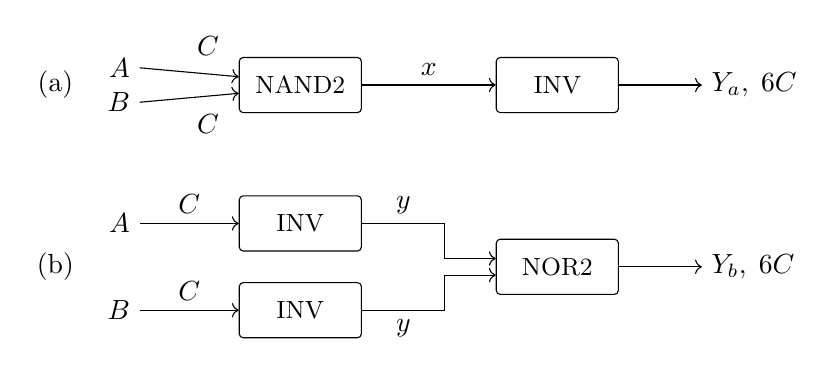
\begin{tikzpicture}[x=1.02cm,y=0.95cm,
      gate/.style={draw,rounded corners=1.4pt,minimum width=1.55cm,
        minimum height=0.7cm,align=center,font=\small}]
    \node at (0.05,1.85) {(a)};
    \node[gate] (nand) at (3.1,1.85) {NAND2};
    \node[gate] (tail) at (6.3,1.85) {INV};
    \draw[->] (1.1,2.08) node[left] {\(A\)}
      -- ([yshift=3pt]nand.west);
    \draw[->] (1.1,1.62) node[left] {\(B\)}
      -- ([yshift=-3pt]nand.west);
    \draw[->] (nand.east) -- (tail.west) node[midway,above] {\(x\)};
    \draw[->] (tail.east) -- (8.1,1.85) node[right] {\(Y_a,\;6C\)};
    \node[above] at (1.95,2.11) {\(C\)};
    \node[below] at (1.95,1.59) {\(C\)};
    \node at (0.05,-0.58) {(b)};
    \node[gate] (invA) at (3.1,0) {INV};
    \node[gate] (invB) at (3.1,-1.16) {INV};
    \node[gate] (nor) at (6.3,-0.58) {NOR2};
    \draw[->] (1.1,0) node[left] {\(A\)} -- (invA.west)
      node[midway,above] {\(C\)};
    \draw[->] (1.1,-1.16) node[left] {\(B\)} -- (invB.west)
      node[midway,above] {\(C\)};
    \draw[->] (invA.east) -- (4.9,0) node[midway,above] {\(y\)}
      |- ([yshift=3pt]nor.west);
    \draw[->] (invB.east) -- (4.9,-1.16) node[midway,below] {\(y\)}
      |- ([yshift=-3pt]nor.west);
    \draw[->] (nor.east) -- (8.1,-0.58) node[right] {\(Y_b,\;6C\)};
  \end{tikzpicture}
  \end{latin}
  \caption{دو پیاده‌سازی \lr{AND} دوورودی، بازترسیم‌شده از
  شکل \secnum{۴.۳۹} کتاب \cite{weste}. \(C\) ظرفیت هر
  ورودی خارجی، \(6C\) بار خروجی، \(x\) ظرفیت ورودی
  \lr{Inverter} پایانی و \(y\) ظرفیت هر ورودی \lr{NOR2}
  است.}
  \label{fig:delay-exercise-and2-paths}
\end{figure}

\textbf{محاسبه تأخیر و اندازه‌ها.}
در \(F=GBH\)، \(F\) همان \lr{Path Effort} و \(G\)
حاصل‌ضرب \lr{Logical Effort} گیت‌های مسیر است. \(B\)
حاصل‌ضرب نسبت بار کل به بار روی مسیر در هر مرحله و
\(H\) نسبت بار انتهایی به ظرفیت ورودی مسیر است.
هر مسیر در هر دو طرح دو مرحله دارد. ظرفیت ورودی همان مسیر
\(C\)، بار خروجی \(6C\) و \(H=6\) است. هر خروجی میانی
فقط یک پایه از گیت بعدی را راه‌اندازی می‌کند، پس \(B=1\).
با \(p=1\) برای \lr{Inverter} و \(p=2\) برای گیت دوورودی، مجموع تأخیر
\lr{Parasitic} در هر دو طرح \(P=3\) است. تفاوت اصلی در
\(G\) است.
با ضرب \(g_i\)های مسیر برای \(G\) و جای‌گذاری در \(F=GBH\) داریم.\[
  G_a=\frac43\cdot1,\quad F_a=8,
  \qquad
  G_b=1\cdot\frac53,\quad F_b=10.
\]
در طرح \lr{(a)}، ترانزیستورهای سریِ گیت دوورودی از نوع
\lr{nMOS} هستند. گیت دوورودی طرح \lr{(b)} برای دستیابی
به قدرت راه‌اندازی مشابه، به \lr{pMOS}های سری عریض‌تر
نیاز دارد. ظرفیت ورودی بیشترِ گیت هم‌قدرت در \(G_b\) بزرگ‌تر
ظاهر می‌شود.
با برابرگرفتن سهم وابسته به بار هر مرحله با \(\sqrt F\)، تأخیرهای
بهینه چنین‌اند.
\[
  D_{\min,a}=2\sqrt{8}+3\approx8.66,
  \qquad
  D_{\min,b}=2\sqrt{10}+3\approx9.32.
\]
ظرفیت هر گیت پایانی با تنظیم سهم وابسته به بارِ آن روی
\(\widehat f=\sqrt F\) به دست می‌آید.
با حل \(g_i C_L/C_{\mathrm{in}}=\widehat f\) برای ظرفیت
ورودی گیت پایانی داریم.\[
  x=\frac{6C}{\sqrt8}\approx2.12C,
  \qquad
  y=\frac{(5/3)6C}{\sqrt{10}}=\sqrt{10}\,C\approx3.16C.
\]
برای کنترل اندازه‌ها، سهم مرحله اول در طرح \lr{(a)}
برابر \((4/3)(x/C)=\sqrt8\) و در طرح \lr{(b)} برابر
\(y/C=\sqrt{10}\) است. بنابراین در هر طرح دو مرحله
\lr{Stage Effort} برابر دارند و برای بار و ظرفیت ورودی
داده‌شده، طرح \lr{(a)} سریع‌تر است.

\clearpage
\begin{thebibliography}{9}
\bibitem{weste}
\begin{latin}
Neil H. E. Weste and David Money Harris,
\textit{CMOS VLSI Design: A Circuits and Systems Perspective},
Fourth Edition, Addison-Wesley (Pearson Education), 2011.
\end{latin}
فصل \lr{Delay}، بخش‌های \secnum{۴.۴} و \secnum{۴.۵}،
صفحات چاپی ۱۵۵ تا ۱۷۳. صورت تمرین‌ها و شکل \secnum{۴.۳۹}
در صفحه چاپی ۱۷۷، برابر با صفحه ۲۰۴ فایل \lr{PDF}، آمده‌اند.
\bibitem{logicaleffortslides}
\lr{Review: Logical Effort}، از مجموعه اسلایدهای \lr{CMOS VLSI Design, Fourth Edition}،
برگرفته از یادداشت‌های \lr{David Money Harris} (۲۰۱۱).
انتساب یادداشت‌های اصلی و توضیح اقتباس در اسلاید ۲ مجموعه
\lr{Introduction} آمده است.
\end{thebibliography}
\end{document}
